	
	\subsection{Présentation UEDF}
	
	Nous avons déjà présenté précédemment \textbf{UEDF}, de façon globale et succincte. 
	Dans cette partie, nous allons détailler \textbf{UEDF} afin d'en avoir une meilleure compréhension. Cela 
	permettra de mesurer la différence entre les attentes théoriques et les résultats obtenus.\newline

	Nous avons évoqué les intérêts de l'implémentation d'\textbf{UEDF} :\\
	Tout d'abord, il est principalement \hyperref[inline]{en ligne}, ce qui n'est pas le cas de 
	la plupart des ordonnanceurs utilisés dans l'industrie.
	Ensuite, il est global. Or, la plupart des ordonnanceurs 
	globaux connus et implémentés ne sont pas optimaux (pour la classe périodique), pour la
	raison exposée au préalable dans ce travail : il est nécessaire d'avoir de la clairvoyance, 
	c'est à dire une connaissance relative du futur.\newline
	
	\subsubsection{Définitions}
	Pour analyser son fonctionnement, nous devons poser quelques définitions. Aussi, par souci de clarté, nous posons que 
	l'offset [\ref*{offset}] de la tâche est nul dans la partie qui suit.\\
	\paragraph{Tâche active}\label{tacheactive}
	Ce qui définit une tâche \og{}active\fg{} peut différer selon le contexte. Dans l'approche d'\textbf{UEDF}, une tâche est 
	considérée comme active si un travail a été relâché et que ce travail n'a pas encore atteint son échéance. 
	Un travail $\tau_i$ est actif s'il a été relâché sur ou avant $t$ et que $d_i(t) \geq t$.
	Une tâche peut donc 
	être considérée comme active même si l'exécution d'un travail en cours est terminée. 
	Concrètement, si une tâche est périodique à échéance implicite [\ref*{echeancesurrequete}], elle est active en permanence dès le 
	premier relâchement de travail. Le travail sera actif durant son relâchement jusqu'à ce que $t \geq d_i(t)$, où 
	une nouvelle instance de la tâche $\tau_i$ sera relâchée.
	
	
	\paragraph{Ensemble des tâches actives}\label{ensembledestachesactives}
	Dans \textbf{UEDF}, on effectue le parcours d'une liste des tâches actuellement actives dans le système, 
	cette liste étant ordonnée par échéances. 
	 L'ensemble des tâches actives est écrit $A(t)$ dans les formules qui suivent.\newline
	
	Pour décrire \textbf{UEDF}, nous allons le décomposer en étapes.
	À chaque fois qu'un nouveau travail est relâché, cela va provoquer le calcul suivant :\newline
	\paragraph{Allot}
	Les tâches actives [\ref*{tacheactive}] sont ordonnées dans une liste. La priorité est définie selon l'échéance, 
	la plus petite étant la plus prioritaire, comme dans \textbf{EDF} [\ref*{EDF}].
	Dans cette phase, l'algorithme va \og{}réserver\fg{} des tranches de temps d'exécution des tâches sur les 
	processeurs, cela en calculant une valeur : \\
	$allot_{ij}$ pour $i \in \{0, nb\_de\_taches - 1\}$, pour $j \in \{0, nb\_processeurs - 1\}$
	La valeur $allot_{ij}$ représente le nombre d'unités d'exécution de la tâche $i$ réservé sur le processeur $j$.\newline
	Si cette valeur est positive, alors le temps $allot_{ij}$ du travail $i$ est réservé sur le 
	processeur $j$. Si cette valeur est égale à $0$, aucun temps n'est réservé 
	à l'exécution de la tâche $\tau_i$ sur le processeur $\pi_j$. Cela permet la constitution d'une liste, 
	\textbf{Eligible}.\newline


	Les calculs sont longuement décrits et expliqués dans la thèse de G. Nelissen \cite{nelissen_u-edf_2012}, aussi nous invitons 
	le lecteur curieux à se référer à ce document pour de plus amples détails. Mais en résumé, 
	ce calcul se déroule de cette façon :
	
	Nous posons :
	\begin{itemize}
		\item $delay = d_i(t) - t$
		\item $ret_i = wcet - $ le nombre d'unités de temps déjà exécutées
		\item $m = $ le nombre de processeurs
		\item L'opérateur $[x]_a^b \defeq \max\{a, \min\{b, x \}\}$
	\end{itemize}


	\label{algouedf}
	\begin{algorithm}[H]
		\caption{Compute Allot}
		\begin{algorithmic}
			\REQUIRE $A(t)$ ordonné par échéances
			\STATE $W = 0$
			
			\FORALL{ $j \leftarrow \{1 ...m\} $}
				\item $RES_j \leftarrow 0$
				\item $ALLOT_j \leftarrow 0$
			\ENDFOR
	
			\FORALL{ $\tau_i \in A(t) $}
				\item $prev_i \leftarrow 0$
				\FORALL{ $j \leftarrow \{1 ...m\} $}
					\item $RES_j \leftarrow RES_j = \{[W]_{j-1}^{j} - (j - 1)\}\times (d_i(t) - d_{i-1}(t))$
					\item $ALLOT_{max} \leftarrow delay - ALLOT_j - RES_j - prev_i$
					\item $allot_{ij} \leftarrow min\{allot_{max}, ret_i - prev_i\}$
					\item $prev_i \leftarrow prev_i + allot_{ij}$
					\item $ALLOT_j \leftarrow ALLOT_j + allot_{ij}$
				\ENDFOR
				\item $W \leftarrow W + U_i$
			\ENDFOR
		\end{algorithmic}
	\end{algorithm}
	
	Dans l'exemple qui suit, notre système est composé de deux tâches :
	\begin{enumerate}
		\item $\tau_1 : \{o:0; w:30; d=p:60;\}$
		\item $\tau_2 : \{o:0; w:60; d=p:80;\}$
	\end{enumerate}
	\begin{figure}[H]
		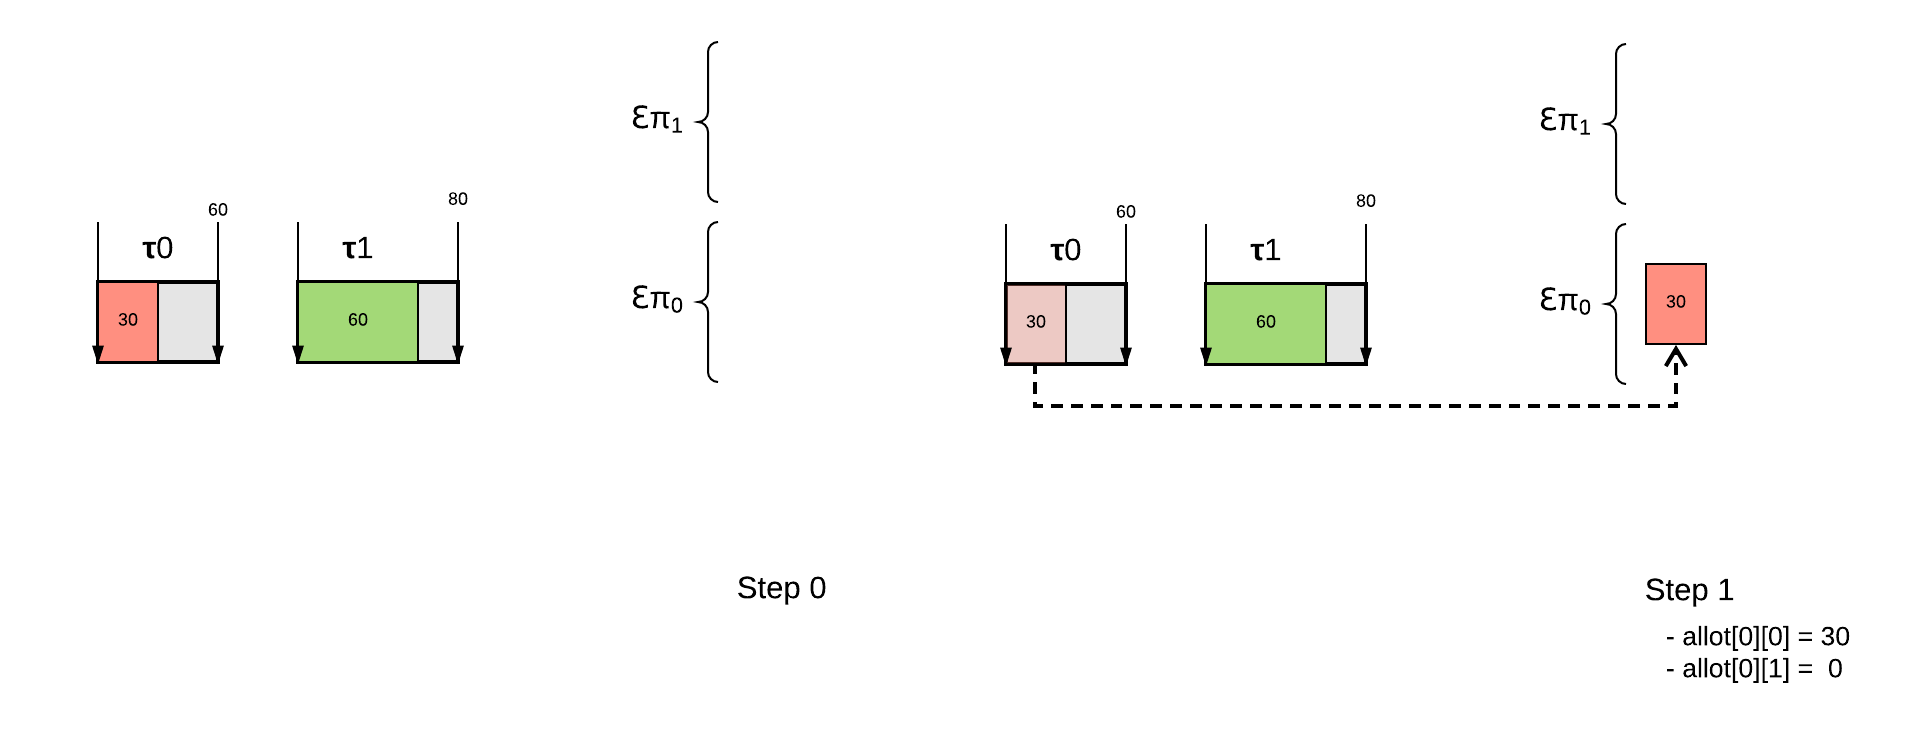
\includegraphics[scale=1]{img/uedf/uedf12}
		\caption{étapes 0 et 1}
		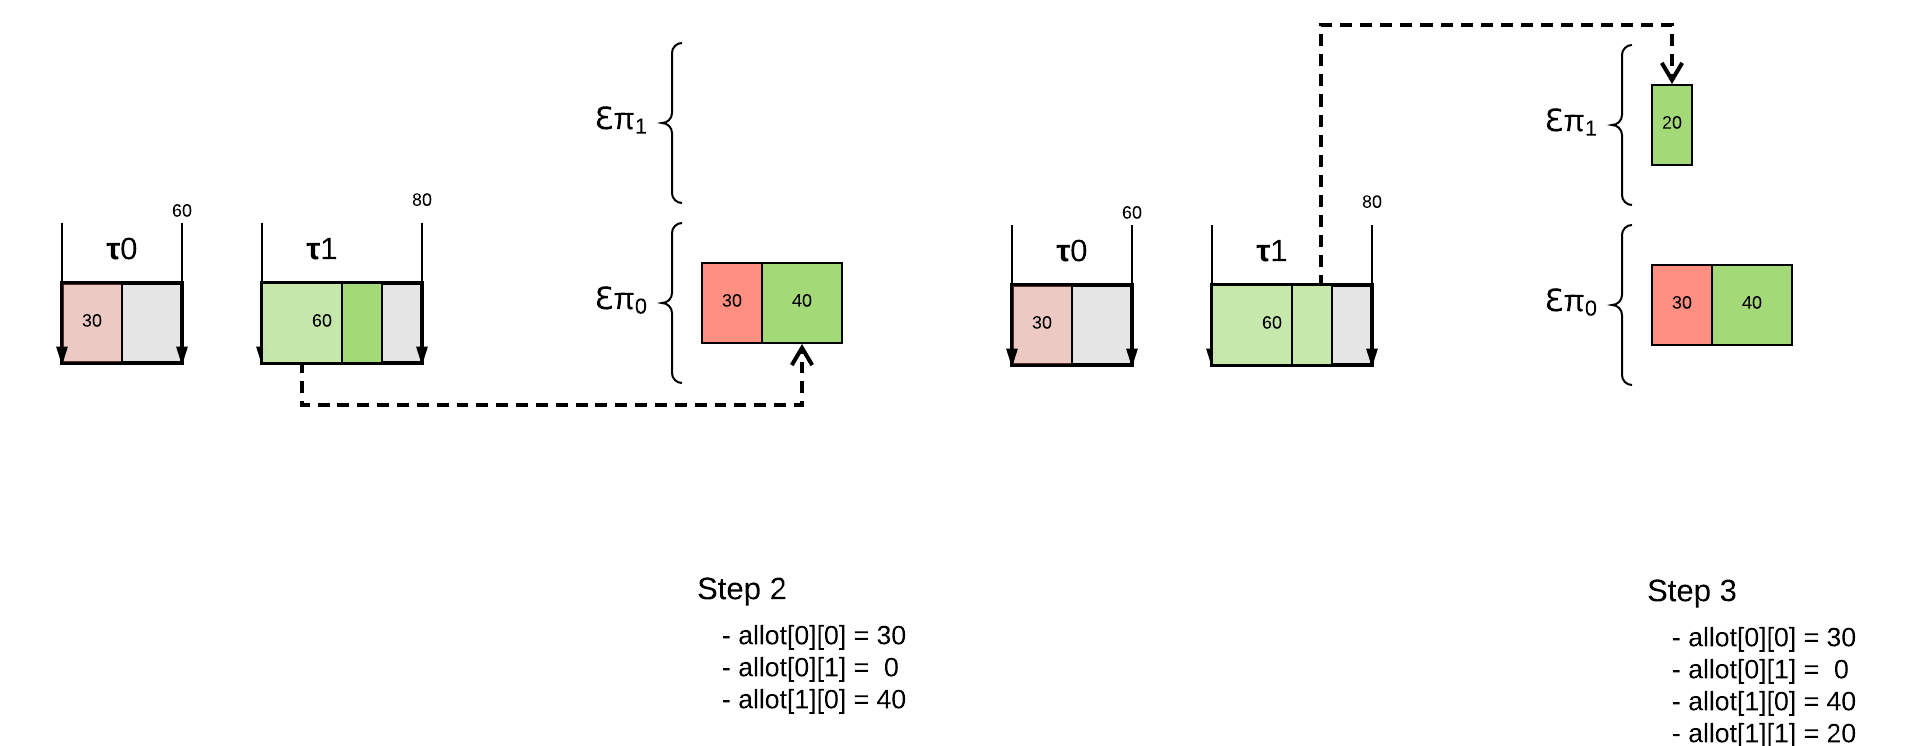
\includegraphics[scale=1]{img/uedf/uedf34}
		\caption{étapes 2 et 3}
	\end{figure}
	\paragraph{Eligible}
	À ce stade, aucune décision d'ordonnancement n'est encore prise, mais des ensembles de tâches (\textit{Eligible}, 
	noté $\epsilon$ dans la suite) sont créés sous forme de listes. Chaque liste \textit{Eligible} définit 
	les seules tâches que les processeurs associés peuvent exécuter (en cela, cette phase d'\textbf{UEDF} peut 
	être considérée comme une phase de partitionnement) durant l'exécution à venir.\newline
	
	Notons que les calculs fournis par l'algorithme permettent en théorie de \og{}remplir\fg{} 
	la charge d'un processeur à 100\% d'utilisation avant de passer au suivant. Concrètement, 
	cela signifie que si la première tâche a une utilisation de moins de 100\%, elle sera suivie par 
	au moins une partie d'une autre.\newline
	
	Les valeurs d'$Allot$ ne doivent pas être considérées comme le temps d'exécution qui sera réellement 
	exécuté sur le processeur. Il faut garder à l'esprit qu'à chaque relâchement de travail, 
	$Allot$ sera recalculé. 

	\paragraph{Prise de décision}
	La phase de décision de l'ordonnancement se déroule lors de la phase suivante.
	\textbf{UEDF} s'inspire pour finir de \textbf{EDF-Delay}. 
	Cet algorithme est très simple :
	\begin{itemize}
		\setlength\itemsep{0.1em}
		\item Une tâche $\tau_i \in \epsilon_j$ est attribuée à un processeur si aucun autre processeur d'index plus bas n'est en train de l'exécuter
		\item $\tau_i$ s'exécute sur le processeur tant qu'$allot_{ij} > 0$.
	\end{itemize}


	\subsubsection{Déroulement}	
	L'algorithme $Compute Allot$ est à effectuer à chaque relâchement de tâche. La valeur $Allot_{ij}$ 
	doit être mise à jour à chaque prise de décision. Une décision est attendue pour chacun des événements suivants :
	\begin{itemize}
		\setlength\itemsep{0.1em}
		\item Une instance de tâche (travail) a été relâchée
		\item Un travail est terminé
		\item $allot{ij} = 0$, pour $i$ un travail et $j$ un processeur 
	\end{itemize}
	
	On peut voir en théorie l'ordonnancement de trois tâches en annexe, afin de mieux comprendre le déroulement d'une exécution.
	À titre de remarque, le travail d'illustration d'une exécution nous semble 
	important pour procéder à une implémentation, sinon le risque est d'omettre le développement 
	d'outils indispensables au bon déroulement de l'exécution. L'algorithme n'est pas évident à mettre en œuvre.
	\todo{gantt chart avec exemple 30;60, 60; 80, 60;80}
	\newline
	
	Nous pouvons déjà formuler ici une nuance par rapport à la théorie et les attentes que l'on peut en avoir 
	en pratique : 
	Nous savons dès le départ que l'algorithme \textbf{UEDF} est assez gourmand en calcul puisque chaque relâchement de 
	tâche va provoquer l'exécution de l'algorithme $Compute Allot$, or, le calcul de cette valeur 
	implique un parcours de toutes les tâches ordonnées, pour chaque processeur. 
	Outre qu'il est nécessaire de gérer une structure de données efficace, nous pouvons 
	déjà considérer que le tri de la structure sera d'un coût non négligeable lors de l'exécution. \newline
	
	Par ailleurs, le calcul même de $Compute Allot$ implique lui aussi une certaine complexité.
	Ainsi :
	\begin{itemize}
		\setlength\itemsep{0.1em}
		\item soit $m$ le nombre de processeurs
		\item soit $n$ le nombre de tâches actives [\ref*{tacheactive}] du système
		\item $Compute Allot \in O(m\times n)$
	\end{itemize}

	Et pour finir, régulièrement, la valeur $allot_{ij} \forall i \in TaskSet, \forall j \in m$ doit être mise 
	à jour, dont la complexité est donc :
	\begin{itemize}
		\setlength\itemsep{0.1em}
			\item soit $m$ le nombre de processeurs
			\item soit $n$ le nombre de tâches actives [\ref*{tacheactive}] du système
			\item $update Allot \in O(m\times n)$
	\end{itemize}

	Nous pouvons attendre un surcoût important sur cette base. Une hypothèse étant que ce surcoût 
	augmente avec le nombre de tâches, mais aussi avec le nombre de cœurs. Un même système pourrait avoir plus 
	de surcoût avec plus de cœurs. Cela pourra être vérifié dans les expérimentations.

	\newpage
	
	
	
	
	
	
	
	
	
	
	
	
	
	
	
	
	
	\subsection{Comparaison avec Global-EDF}
	
	Nous avons choisi de comparer \textbf{UEDF} à \textbf{Global-EDF} [\ref*{GlobalEDF}]. 
	La raison de ce choix est simple : 
	cet algorithme est implémenté sur le RTOS HIPPEROS et il est global, comme 
	l'indique son nom. 
	Les autres ordonnanceurs disponibles sur HIPPEROS sont pour la plupart partitionnés.
 
	Aussi les tests effectués sur \textbf{UEDF} seront également faits en utilisant \textbf{Global-EDF} pour 
	élément de comparaison.\newline
	
	Ces deux algorithmes ont toutefois de grandes différences. \textbf{Global-EDF}
	ne permet pas -- même théoriquement -- d'atteindre l'optimalité. Ceci s'explique par le fait que 
	\textbf{Global-ED}F peut être considéré comme \og{}vertical\fg{} là où \textbf{UEDF} serait \og{}horizontal\fg{}, et ce faisant, 
	n'a pas de \og{}vision de l'avenir\fg{}, autrement nommée \og{}clairvoyance\fg{}.
	
	\subsubsection{Fonctionnement de Global EDF}
	
	L'algorithme est relativement simple, et pour les besoins de la comparaison, nous résumons 
	ici son fonctionnement.\\
	À un moment \textit{t}, l'ordonnanceur prend sa décision de cette façon :
	si un processeur est libre, il se voit attribué le travail de priorité supérieure parmi 
	tous les travaux actifs. Cela permet d'avoir un algorithme peu gourmand.
	
	\begin{algorithm}
	\caption{Global-EDF}
	\begin{algorithmic}
		\REQUIRE $JobSet(t)$ ordonné par échéances
		\FORALL{ $j \in m $}
			\item $decision \leftarrow pop(JobSet(t))$
		\ENDFOR
	\end{algorithmic}
\end{algorithm}	
	
	L'algorithme permet de prendre une décision au moment \textit{t} en ne considérant 
	que les travaux à exécuter par ordre de priorité et les processeurs disponibles.
	
	Si l'on reprend l'exemple illustré précédemment, la décision sera prise de cette façon :\newline
	
	
	\begin{figure}[H]
		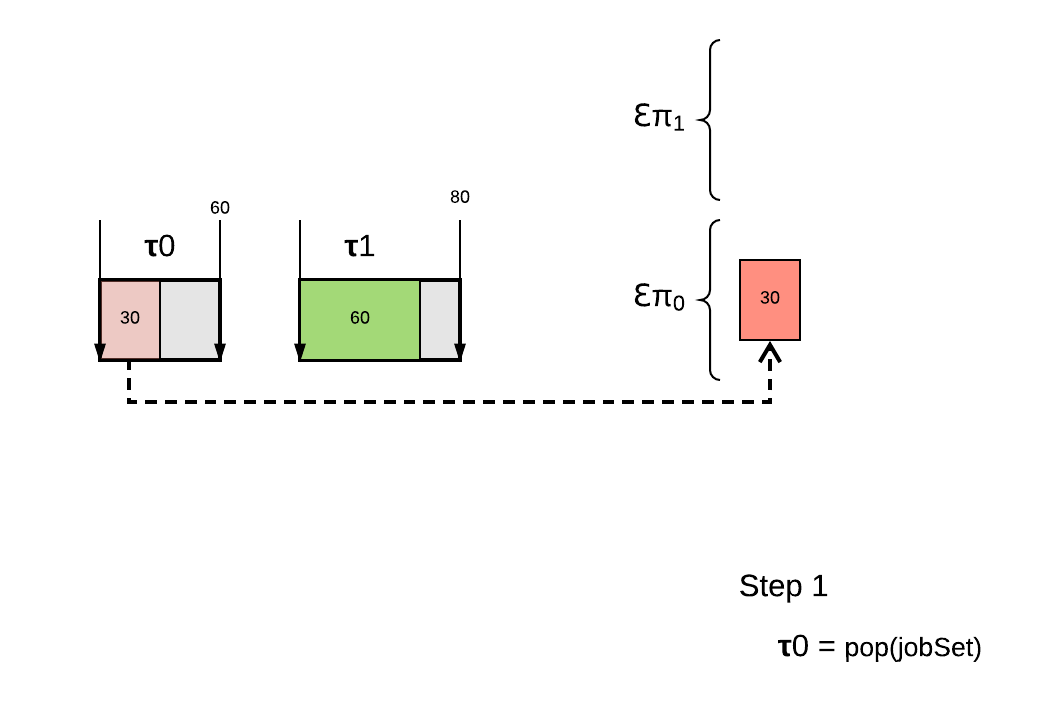
\includegraphics[scale=0.5]{img/gedf/gedf}
		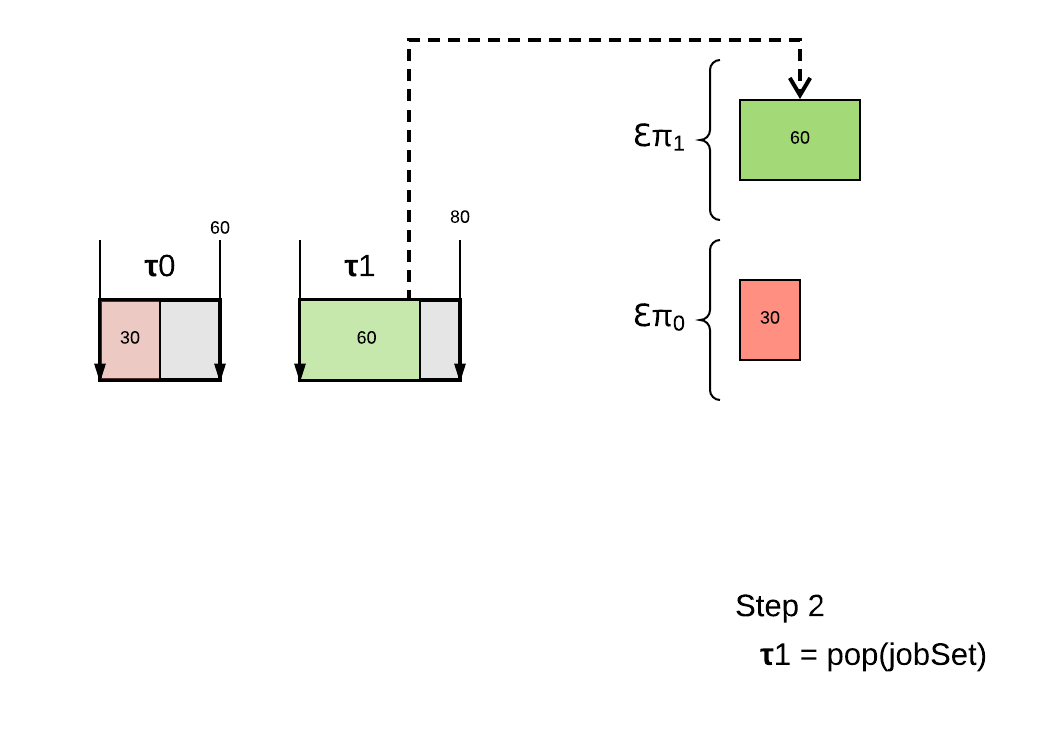
\includegraphics[scale=0.5]{img/gedf/gedf2}
		\caption{Global EDF}
	\end{figure}
	 
	On peut facilement voir que cela peut entraîner de \og{}mauvais choix\fg{}. 
	En changeant l'exemple précédent, et en prenant un exemple avec 3 travaux, 
	on n'obtiendra pas du tout le même ordonnancement dans les deux algorithmes, 
	et celui-ci mettra en échec \textbf{Global-EDF} quasiment immédiatement.\newline
	
	Prenons un ensemble de trois tâches comme suit :

	\begin{enumerate}
		\setlength\itemsep{0.1em}
		\item $\tau_1 : \{o:0; w:40; d=p:60;\}$
		\item $\tau_2 : \{o:0; w:40; d=p:60;\}$
		\item $\tau_3 : \{o:0; w:40; d=p:60;\}$
	\end{enumerate}
	
	\todo{insérer schema ici}
	
	Malgré ce point, \textbf{Global-EDF} est \og{}efficace\fg{} en terme de calculs.
	Le point le plus complexe concerne la structure de données qui conserve les 
	tâches courantes. Une bonne idée est d'utiliser un Heap [\ref*{heap}] qui 
	va permettre de fournir toujours en tête le travail de priorité supérieure.
	Pour s'assurer de la faisabilité de l'ensemble de tâches, 
	il faudra tester l'ordonnancement suffisamment longtemps (hyper-période).\newline
		
\section{HIPPEROS}
	\customhighlight{HIPPEROS} (\textbf{HI}gh \textbf{P}erformance \textbf{P}arallel \textbf{E}mbedded \textbf{R}eal-time \textbf{O}perating \textbf{S}ystems)
	est un \customhighlight{RTOS} (Real-Time Operating System) développé depuis plusieurs années par une spinoff de l'ULB.
	Il bénéficie des connaissances apportées par le monde de la recherche dans 
	le domaine des systèmes critiques avec multic\oe{}urs. Une de ses particularités 
	est sa modularité, qui permet d'adapter ses possibilités en fonction du système 
	lors de la compilation de l'OS, ainsi peut-on différencier principalement 
	deux installations en fonction des particularités. 
	
	\customhighlight{HIPPEROS} est un candidat idéal pour l'implémentation d'un ordonnanceur 
	global. Il a cependant un fonctionnement propre qui pourra rendre l'implémentation 
	plus ou moins facile, et poser un certain nombre de problèmes. 
	En résumé, une nouvelle implémentation sur un OS différent 
	peut elle-aussi apporter à la connaissance générale des détails importants.
		

\section{Implémentation}

	Dans cette partie, nous allons analyser les difficultés rencontrées lors de l'implémentation en elle-même, 
	en nous concentrant sur celles liées aux aspects théoriques d'origine. 

	\subsubsection{Données temporelles}
	
		Dans \textbf{HIPPEROS}, il existe plusieurs ordonnanceurs déjà implémentés. 
		Ils ont leur fonctionnement propre, et de façon générale, sont assez différents d'\textbf{UEDF} par 
		rapport aux variables auxquelles ils accèdent. 
		UEDF a besoin de l'\textit{utilisation} d'une tâche dans certains de ses calculs. Or, l'\textit{utilisation} 
		est une fraction. Nous souhaitons éviter la représentation à virgule flottante 
		pour gérer ces fractions, et par conséquent, cela nécessite un décalage des valeurs.\newline
		 
		Se pose immédiatement la question de combien peut-on décaler le WCET et la période afin d'avoir le moins de pertes possibles. 
		La réponse à apporter diverge en fonction de plusieurs facteurs :
		\begin{itemize}
			\setlength\itemsep{0.1em}
			\item Comment sont stockées les valeurs temporelles $period$ et $wcet$ ? Des entiers non signés sur $64$ bits
			\item Quel type de valeurs peut-on avoir pour une utilisation ? Nous négligeons celles de moins de $1 \%$, 
			une tâche peut avoir une utilisation de $1$ à $100\%$.
			\item Quelles valeurs pouvons-nous atteindre ? Pour 4 processeurs, $400\%$.
			\item quelle sera l'incidence de cette valeur dans les calculs ? Si l'on reprend l'algorithme en section \ref{algouedf}, 
			l'utilisation multiplie la différence entre deux échéances de travaux différents, afin 
			d'en obtenir une proportion. 
		\end{itemize}
		Dans le cas présent, nous avons estimé que décaler les valeurs de $1000$ était un bon compromis. 
		
	\subsection{Structures de données}
		Dans ses nombreux calculs, \textbf{UEDF} fait appel à un certain nombre de données concernant les tâches ou les travaux.
		L'ordonnanceur a également besoin d'accéder à des variables qui lui sont 
		spécifiques à divers moments de l'exécution.\newline
		
		\paragraph{Allot}
		La valeur $Allot$ est primordiale et doit être conservée durant l'exécution, 
		puisqu'elle sera mise à jour à chaque événement.
		Ainsi, on doit conserver un tableau à deux dimensions $Allot$, qui contient des données 
		temporelles (entiers non signés de $64$ bits). 
		Cette structure est de taille $m \times n$ en théorie. 
		En pratique, dans HIPPEROS, $m$ et $n$ sont des valeurs prédéfinies 
		dans chaque version. Le nombre de tâches peut être à ce jour $32$, $128$ ou $1024$.
		Il ne nous a pas semblé utile de changer cela. Nos tests ont tous pour configuration 
		un nombre de tâche maximum de 32.
		\newline
		
		\paragraph{Liste triée de tâches}
		Il est nécessaire de maintenir à jour un ensemble trié de tâches, pour le 
		calcul d'$Allot$. Pour cette structure, notre choix a beaucoup évolué au cours du temps. 
		La première idée était le besoin de parcourir cette liste dans l'ordre, plusieurs fois, 
		d'y ajouter et d'en retirer des éléments. A priori, pour ces raisons, le Heap ne 
		correspond pas bien à nos besoins, aussi avons-nous utilisé une liste liée en 
		premier lieu. Néanmoins, les mauvaises performances de la liste liée 
		nous ont amené à reconsidérer ce choix, d'autant plus que les parcours de listes étaient nombreux. 
		À l'heure actuelle, notre implémentation construit un Heap avant le recalcul d'$Allot$.
		Ce Heap est copié chaque fois avant d'en faire le parcours, dans les diverses parties du code.
		En pratique, lorsque des travaux sont relâchés, nous parcourons à l'heure actuelle 3 fois ce Heap, 
		chaque fois copié au préalable. 
		Ce choix a fait diminuer drastiquement le surcoût.
		\todo{ajouter citation qui dit qu'il faut pas optimiser avant d'avoir bien implémenté, knuth}
		Notons qu'il est tout à fait imaginable de ne pas reconstruire le Heap à chaque fois qu'il faut 
		calculer $Allot$, il faudrait conserver le Heap, et mieux gérer les ajouts ou retraits. C'est 
		une amélioration simple qui n'a pas encore été faite, et pourrait réduire légèrement les surcoûts.
		\todo{ptete essayer avant la remise, ça pourrait se faire facilement je pense.} 
		\newline
		
		\paragraph{Liste d'états}
		Une première chose à laquelle il faut être attentif est de rendre possible les accès 
		aux données, par exemple en conservant des tableaux de références, afin de minimiser les temps 
		d'accès. Cela nécessite de faire un choix : on optimise le temps d'accès en conservant plus de données. 
		L'ordonnancement en cours est ainsi doublement référencé : 
		\begin{itemize}
			\setlength\itemsep{0.1em}
			\item $Job\_id \leftarrow coreToSchedule_{core}$ permet d'obtenir le travail en cours d'exécution sur le processeur $core \in m$
			\item $core \leftarrow scheduledToCore_{job\_id}$ permet d'obtenir le processeur qui exécute le travail $job\_id \in n$.
		\end{itemize}

		Nous devons également conserver les divers états d'un travail. En effet, rappelons que dans \textbf{UEDF}, 
		un travail est considéré comme \textit{actif} tant qu'il n'a pas rencontré son échéance -- et ce, 
		même s'il est \textit{terminé}. Nous conservons donc un tableau d'états permettant 
		d'accéder facilement à cette information.
		De même, nous devons différencier l'état \textit{bloqué} d'un travail \textit{terminé}, ce qui n'est pas le cas 
		dans les autres ordonnanceurs implémentés dans HIPPEROS. Par exemple, dans \textbf{Global-EDF}, si un travail 
		attend une ressource, elle sera purement et simplement retirée de la liste de tâches actives, et lorsqu'elle 
		sera réactivée, elle sera réintroduite dans cette liste. Ce comportement n'est pas possible dans \textbf{UEDF}, 
		qui \og{}réserver\fg{} du temps, et \og{}prévoit\fg{} un ordonnancement. Si le travail sort, et est simplement 
		réintroduit, cela provoquerait un nouveau calcul d'$Allot$, basé sur le $WCET$, et pas le temps restant d'exécution.
		
		\paragraph{WCET, et Temps d'exécution}
		
		Les autres ordonnanceurs implémentés dans HIPPEROS n'utilisent pas les données concernant le temps 
		d'exécution de la tâche dans leur prise de décision. 
		Pour \textbf{UEDF}, nous avons besoin d'un accès efficace et correctement mis à jour à ces données. 
		Typiquement, le \textbf{Temps d'exécution restant}(\textbf{RET}) est utilisé pour le calcul et la mise à jour 
		d'\textbf{Allot}.\newline
		
		En pratique, \textbf{HIPPEROS} met à jour le temps exécuté d'un travail lors d'un événement qui le concerne. 
		Ainsi, si un travail est effectué, on note le moment où le travail a été dispatché.
		Au temps \textit{t}, si l'on veut savoir combien de temps a déjà été exécuté, 
		s'il n'a pas croisé d'événement, il faudra calculer ce temps dans \textbf{UEDF} 
		car \textbf{HIPPEROS} n'aura pas encore mis à jour cette donnée.\newline
		Si en terme de temps d'accès, cette requête n'est pas très compliquée, il n'en demeure pas moins 
		que le résultat sera un peu approximatif, puisque l'ordonnanceur n'arrête pas l'exécution des tâches pendant 
		son exécution. Cela ne change pas fondamentalement le calcul car cela change des valeurs très faibles, 
		mais cela constitue une adaptation de la théorie en pratique.\newline

	\subsubsection{Modèle séquentiel}
	
		Le problème que nous venons d'évoquer plus haut concernant le \textbf{RET}. 
		Dans une siuation modélisée, l'exécution s'arrête, l'algorithme d'ordonnancement est effectué, 
		puis les travaux sont dispatchés et l'exécution reprend.\newline
		 
		Un ordonnanceur fait bien souvent partie des tâches lui-même, et il faut qu'il soit lui-même ordonnancé, 
		afin de pouvoir changer l'exécution en cours. Toujours est-il qu'en attendant, l'exécution sur les autres cœurs 
		n'est pas stoppée, et les données continuent d'évoluer. 
		\todo{NON c'est FAUX !!}
		
		\todo{expliquer dispatcher model :}
		le dispacther demande le schedule, 
		le schedule est calculé, et retourné,
		le dispatcher exécute.
		les événements sont créés : block, kill, activate... et provoquent kill ou activate, donc faut 
		savoir pourquoi on se retrouve dedans computeSchedule.

		Si un ou des nouveaux travaux : un booléen indique qu'il faut recalculer Allot. Puis, 
		on fait l'assignation ensuite.
		S'il n'y a pas de nouveaux travaux mais qu'il y a un ou des travaux terminés :
		pour chaque processeur libre, prendre une décision pour la suite.\newline
		
		C'est aussi simple que ça, mais cela n'est pas décrit dans le papier et représente une 
		adaptation du modèle.
	
		\todo{chart représentant le déroulement d'une exécution ??}
	
		
	\subsubsection{WCET}
		\todo{dev beaucoup plus}
		Le \textbf{WCET}, dans UEDF, est une donnée centrale. Elle est utilisée dans beaucoup de calculs, et 
		son importance est grande pour le résultat. Or, cette donnée n'est pas évidente à produire. \newline
		
		Notre travail nous amène à nous pencher sur ce sujet, qui dépasse largement la portée de ce travail. 
		Néanmoins, voici ce que l'on peut retenir pour nos besoins :\\
		Ce sujet est documenté dans la littérature scientifique. Il n'est pas évident de déterminer le 
		\textbf{WCET} pour toutes les tâches. Mettons qu'une tâche doive faire des lectures/écritures, 
		ce temps-là devra être considéré. Il est possible de déterminer le nombre d'instructions, 
		et donc un temps théorique en fonction de la machine utilisée pour l'exécuter, mais cela dépend 
		parfois de l'exécution. En effet, certaines opérations, en fonction des données, ne vont pas prendre 
		le même temps, or, ce que l'on cherche à déterminer et le pire des cas.\newline
	
		Pour les besoins de ce travail, nous avons simplifié la question, considérant des tâches 
		non dépendantes les unes des autres, avons fait un calcul à la main pour évaluer le 
		nombre d'opérations, et avons vérifié le temps d'exécution des tâches en exécutant un grand nombre 
		de fois les tâches et pris le pire temps comme valeur de \textbf{WCET}. Cela ne garantit en fait 
		pas que le \textbf{WCET} soit réellement le pire des cas, mais cela est suffisant pour nos besoins ici.
	
	\newpage
	\todo{Revoir, c'est DE LA MERDE}
	\subsubsection{Utilisation instantanée et interruptions}

	L'algorithme d'ordonnancement d'\textbf{UEDF} utilise comme variable l'utilisation instantanée du système. 
	Pour rappel, celle-ci est définie par la somme des utilisations des tâches actives à l'instant $t$, 
	tâche active signifiant tâche ayant relâché un travail qui n'a pas encore atteint son échéance. 
	On considère donc ici pouvoir comptabiliser tous les processus en exécution. Ceci est 
	en fait assez théorique et pose certains problèmes.
	
	Le problème de l'évaluation du \textbf{WCET} posé précédemment, il faut à ce stade rappeler comment 
	fonctionne un système d'exploitation.
	
	D'un point de vue théorique, si l'on estime voir l'ensemble des tâches dans un ensemble uniforme, 
	en pratique, ce n'est pas forcément le cas. Dans ce travail, une partie de la complexité est 
	donc éloignée. NUMA = non-memory-uniform-access
	
	Linux traite chaque processus comme un thread. Les threads ont un domaine. 
	https://lwn.net/Articles/80911/
	https://hal.archives-ouvertes.fr/hal-01295194/document  sur le scheduler linux
	\todo{développer cette partie et sourcer}
	

	L'ordonnanceur n'est pas compté dans les tâches, c'est un module du kernel. Par conséquent, il n'est pas comptabilisé 
	dans l'utilisation instantanée. Il fait partie de ce tas que l'on nomme \og{}overhead\fg{} et dans lequel 
	on met tout ce qui prend du temps sans être régulier. 
	Migrations, ordonnanceur, interruptions... Ces temps ne font pas partie du système, mais ils occupent
	pourtant du temps.
	
	Ce n'est pas la seule tâche qui n'est pas comptabilisée dans l'ensemble, puisqu'on peut définir des 
	interruptions côté utilisateur. 
	Concrètement, on imagine une sonde qui envoie très rarement des données. On ne réserve 
	pas de temps, on vérifie régulièrement qu'elle a des données à traiter, et si c'est le cas, on les traite.\\
	C'est un cas d'utilisation du system domain : garantir que les données seront traitées vite, dès qu'elles arrivent, 
	mais ne pas attribuer une tâche pour le faire régulièrement.
	Dans un système d'exploitation, l'ordonnanceur est chargé d'ordonnancer les tâches selon leurs priorités. 
	Pour ce faire, la norme \textbf{POSIX} définit des niveaux de priorité pour les threads. 
	\textbf{HIPPEROS }se base sur la même approche, et définit plusieurs niveaux également. C'est ainsi 
	qu'un thread peut être de scope system, et dans ce cas, sa priorité est haute, ou de priorité 
	moindre, et il sera ordonnancé par \textbf{UEDF}.\newline
	
	Tout ceci montre les limites d'un modèle où l'on charge l'utilisation des processeurs à 100\% avant de 
	passer au suivant. Certes, l'utilisation sera optimisée, dans le sens où l'on 
	pourra utiliser moins de processeurs, mais en revanche, on 
	répartir moins bien la somme de travail, et atteint très vite une somme critique pour les processeurs utilisés.
